\documentclass[a4paper, 11pt, titlepage, oneside]{report}
\usepackage[utf8]{inputenc}
\usepackage[T1]{fontenc}
\usepackage{graphicx}
%\usepackage{caption}
%\usepackage{subcaption}
\usepackage{verbatim}
\usepackage[margin=1in]{geometry}
\usepackage[french]{babel}
\usepackage{hyperref}
\usepackage{xcolor}
\usepackage{framed}
% \usepackage{tcolorbox}
\usepackage{titlesec}
\usepackage[toc, page]{appendix}
\usepackage{listings}
\usepackage[acronym,toc,section=chapter,sanitize={name=false,description=false,symbol=true}]{glossaries}
\usepackage{float}
\usepackage{pgf}
\usepackage{tikz}
\usepackage{pgfplots}
\usetikzlibrary{automata, arrows}
\usepackage{amsmath, amsthm, amssymb, mathtools}

\usepackage{array}
\newcolumntype{P}[1]{>{\centering\arraybackslash}p{#1}}

\usepackage{afterpage}
\newcommand\blankpage{%
    \null
    \thispagestyle{empty}%
    \addtocounter{page}{-1}%
    \newpage}

\graphicspath{{figures/}}
\setkeys{Gin}{width=\linewidth}
\setlength{\parindent}{1em}
\setlength{\parskip}{1em}

\lstset{%
    frame=single,
    basicstyle=\footnotesize\ttfamily,
    numbers=left,
    stepnumber=1
}

\renewcommand{\appendixtocname}{Annexes}
\renewcommand{\appendixpagename}{Annexes}

\titleformat{\chapter}
  {\normalfont\LARGE\bfseries}{\thechapter}{1em}{}
\titlespacing*{\chapter}{0pt}{3.5ex plus 1ex minus .2ex}{2.3ex plus .2ex}

\frenchbsetup{IndentFirst=false}

% \defglsdisplayfirst[main]{#1#4\protect\footnote{#2}}
% \makeglossaries
% \newglossaryentry{JSON}{
%     name={JSON},
%     description={JavaScript Object Notation (JSON) est un format de données textuelles dérivé de la notation des objets du langage JavaScript. Il permet de représenter de l’information structurée comme le permet XML par exemple.}
% }
% }

\begin{document}
    \begin{titlepage}
    \begin{center}
        \vspace*{2cm}
        \hrule width \hsize height 2pt 
        
        % 
\includegraphics[width=0.25\linewidth]{logo.png}\\[1.5cm]
        \large{\textbf{Pas de jaloux}}\\[0.35cm]
        \textbf{\LARGE Cahier des charges} \\ [0.7cm]
        
        \hrule width \hsize \kern 1mm \hrule width \hsize height 2pt
        \vspace{0.7cm}
        
        % % -- AUTHORS
        \begin{center}
        		\textit{Contacts}\\[0.5cm]
        		Nicolas Maudet \texttt{(nicolas.maudet@lip6.fr)} \\
			Aurélie Beynier \texttt{(aurelie.beynier@lip6.fr)}\\[1cm]
			
			\textit{Équipe prestataire}\\[0.5cm]
			Thirunavukarasu Hans \texttt{(hans.thiru@gmail.com)}\\
			Bontems Alexandre \texttt{(alexandre.bontems@gmail.com)}\\
			Mottola Gualtiero \texttt{(gualt1995@gmail.com)}

        \end{center}
        \vfill
        % % -- ADDRESSES
        \begin{minipage}{0.5\textwidth}
            \small
            Université Pierre et Marie Curie, Paris 6,\\
            Département Informatique \\
            4 place Jussieu 75252 Paris cedex 05, France\\
        \end{minipage}~
        \begin{minipage}{0.5\textwidth}
            \flushright
            
\includegraphics[width=0.5\linewidth]{sorbonne.png}
        \end{minipage}
    \end{center}
    \end{titlepage}

    \tableofcontents
%    \thispagestyle{plain}
    
    \chapter{Présentation du projet}
    
    L’idée, dans ce projet, est de développer un jeu mobile basé sur le problème de partage équitable suivant:
    
\textit{n agents sont alignés sur une ligne et disposent de n objets en face d’eux. Il faut assigner un objet différent à chaque agent en fonction de leur préférence tout en prenant en compte la notion de jalousie. Si un agent voit que l’un de ses voisins (à gauche ou à droite) s’est vu attribuer un objet qu’il préfère à celui qu’il possède, alors on dira qu’il est jaloux et que l’affectation n’est pas valide.}

	\begin{figure}[h!]
		\centering
		\begin{tabular}{P{2.1cm} P{2.1cm} P{2.1cm} P{2.1cm}}
		2 & 2 & \colorbox{yellow}{1} & 4 \\
		\colorbox{yellow}{3} & \colorbox{yellow}{4} & 2 & 3 \\
		4 & 1 & 3 & \colorbox{yellow}{2} \\
		1 & 3 & 4 & 1
		\end{tabular}\\[0.15cm]
		\begin{tikzpicture}[node distance=2.5cm, semithick]
			\node[state] (a) {a};
			\node[state] (b) [right of=a] {b};
			\node[state] (c) [right of=b] {c};
			\node[state] (d) [right of=c] {d};
			
			\path (a) edge node {} (b)
				  (b) edge node {} (c)
				  (c) edge node {} (d);
		\end{tikzpicture}
		\caption{Exemple d'instance à 4 agents et 4 objets}
		\label{fig:ex-instance}
	\end{figure}
	
	Dans l’exemple de la figure~\ref{fig:ex-instance}, les objets sont triés par ordre de préférence pour chaque agent (le plus haut étant le préféré) et une affectation possible sans jaloux est surlignée. On remarque que l'on ne peut pas affecter l'objet 2 aux agents $a$ et $b$ sans créer de jalousie par exemple.
	
	\section{Objectifs}
	
	Ce projet s’inscrit dans le cadre de l’UE Projet du master ANDROIDE et demande de l’équipe prestataire l’application des méthodes d’optimisation apprises au sein de la formation afin de permettre l’analyse du problème exposé ci-dessus. Plus précisément, il s’agit de:
	\begin{itemize}
		\item Déterminer la solvabilité d’une instance.
		\item Évaluer la difficulté de résolution d’une instance.
		\item Obtenir des instances de difficultés variées.
	\end{itemize}
L’équipe prestataire est ainsi amenée à explorer des problématiques de modélisation et d’analyse de problèmes NP-difficiles avec pour objectif de trouver des heuristiques portant sur la difficulté de résolution du problème.

Dans un second temps, le développement d’un jeu mobile basé sur le problème est demandé. Les principaux résultats suivants sont attendus:
\begin{itemize}
	\item Pouvoir jouer/résoudre une instance d’une certaine difficultée.
	\item Pouvoir jouer avec plusieurs instances successives selon une courbe de progression (difficulté augmentante, variantes de jeu, etc).
\end{itemize}

	\section{Analyse du problème}
	
	Afin de proposer au sein de l’application des enjeux intéressants pour les joueurs, le projet devra répondre aux spécifications suivantes:
	\begin{itemize}
		\item Obtention d’instances solvables. 
		\item Développement d’outils permettant d’évaluer la difficulté de résolution d’une certaine instance. 
	\end{itemize}
On aimerait à terme intégrer les instances évaluées dans l’application mobile. Elles correspondront donc soit à des instances générées aléatoirement et qui auront pu être évaluées, soit à des instances générées procéduralement si possible. Une partie de l’analyse sera donc dédiée à la recherche des caractéristiques associées à la difficulté des instances.

Puisque les résultats sont destinés à être utilisés en tant qu'indicateurs pour une résolution par l'humain, on s'intéressera également aux méthodes de résolution du problème "à la main".

Plusieurs extensions du jeu seront considérées:
\begin{itemize}
	\item Possibilité d’échanger la position de deux agents,
	\item Possibilité d’obstruer la vision entre deux agents et donc d’éliminer toute jalousie possible entre eux,
	\item Plus d’un type d’objet possible; les agents se voient alors attribuer plus d’un objet et précisent des préférences pour chaque type différent.
\end{itemize}

	\section{Application mobile}
	\label{sec:app}
		\subsection{Besoins fonctionnels: front-end}
		
L’interface de l’application mobile devra comprendre les éléments suivants:
\begin{itemize}
	\item Menu principal.
	\item Menu options.
	\item Sélection des niveaux.
	\item Écran dédié au jeu.
\end{itemize}

Elle devra aussi répondre aux problématiques principales suivantes: 
\begin{itemize}
	\item Gestion de l’encombrement de l'écran lorsque le nombre d’agents devient important; comment gérer les défilements ?
	\item Facilitation de la lecture de l’information (code couleurs, organisation de l’espace, ...).
\end{itemize}\

Afin de consolider les résultats de l’analyse, on envisage l’intégration d’une fonctionnalité de retour utilisateur pour la difficulté ressentie des niveaux.

Proposer une charte graphique accueillante pour les joueurs et permettant une compréhension optimale du problème fait également partie des objectifs principaux.

	\subsection{Besoins fonctionnels: back-end}
	
	En ce qui concerne les besoins fonctionnels de l’application, outre une architecture répondant aux spécifications front-end, il est surtout intéressant de détailler la gestion des niveaux. En fonction de l’évolution de l’analyse, deux possibilités sont envisagées:
	\begin{enumerate}
		\item Génération des niveaux sur le terminal selon des règles de générations résultantes de la première partie du projet. On pourrait ainsi offrir une grande rejouabilité.
		\item Stockage des niveaux sous forme de fichier XML qui seront alors générés et évalués en amont.
	\end{enumerate}

	Dans les premiers jours de l'application, une fonctionnalité d'enregistrement des actions utilisateurs sera inclue (dans le cadre de l'analyse des méthodes de résolution du problème par l'humain). On cherchera à extraire les intuitions qu'utilisent les joueurs pour trouver une solution et quelles caractéristiques du problèmes pourraient rendre une instance difficile face à ces intuitions.

	\subsection{Spécifications logicielles}
	
	L’application sera développée pour la plateforme Android sous Android Studio, elle sera compatible avec tous les terminaux sous android 6.0 ou plus, la distribution du software se fera au travers de la plateforme Google Play. Le langage utilisé pour la logique de l’application sera le Java.

	\chapter{Prestations attendues}
	\section{Développement}
	
	
	Une méthodologie de développement agile sera mise en place avec rendez-vous réguliers avec les clients (hebdomadaires la plupart du temps). 

Un suivi de la progression sera possible grâce à un repository Github dédié sur lequel seront déposés tous les codes et documents produits.

	\section{Maquette de l'application}
	
	Les figures~\ref{fig:mockup1} et~\ref{fig:mockup2} présentent un layout basique qui sera développé en profondeur lors de la phase de conception.

	\begin{figure}[h!]
		\centering
		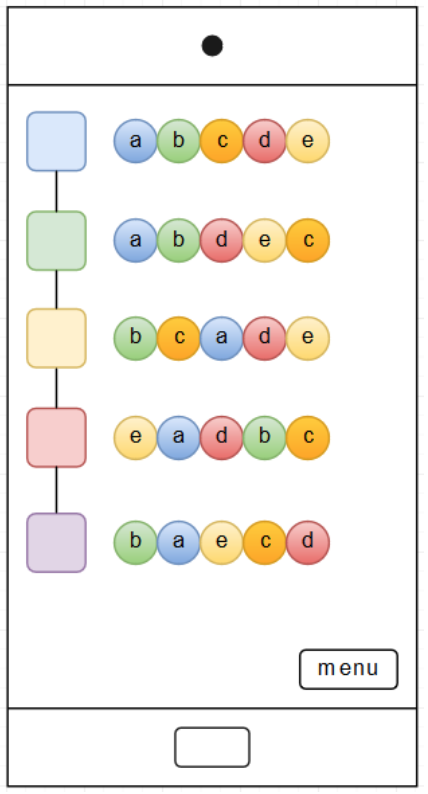
\includegraphics[width=0.3\linewidth]{maquette.png}
		\caption{Maquette conceptuelle de l'application}
		\label{fig:mockup1}
	\end{figure}
	
	\begin{figure}[h!]
		\centering
		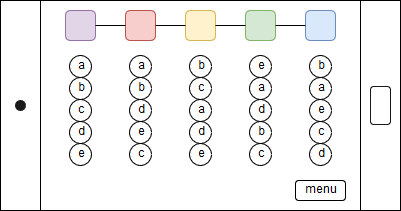
\includegraphics[width=0.7\linewidth]{maquette2.png}
		\caption{Maquette conceptuelle de l'application}
		\label{fig:mockup2}
	\end{figure}
	
	\section{Documentation}
	
	La production d’une documentation utilisateur est demandée. Elle concernera aussi bien toute application permettant l’évaluation des instances du problème que l’application mobile décrite en~\ref{sec:app}.
	
	\section{Livrables attendus}
	
	Les objets suivants devront être produits pour les clients:
	\begin{itemize}
		\item Documentation.
		\item Document de recherche.
		\item Sources de l’analyse.
		\item Sources de l’application mobile.
	\end{itemize}
	
	\section{Planification}
	
	\begin{center}
		\begin{tabular}{|c|c|}
			\hline
			\textbf{Livrable} & \textbf{Échéance} \\
			\hline
			Cahier des charges & 5 mars 2018 \\
			Application v0 (à faire circuler en groupe réduit) & 12 mars 2018 \\
			... & ... \\
			Rapport de projet & 25 mai 2018 \\
			\hline
			
		\end{tabular}
	\end{center}

\end{document}
